\section{Theory}
\fboxsep=1mm%padding thickness
\fboxrule=1pt%border thickness

\begin{figure*}[t]
    \centering
    %  trim={<left> <lower> <right> <upper>}
    %\fcolorbox{red}{yellow}{
        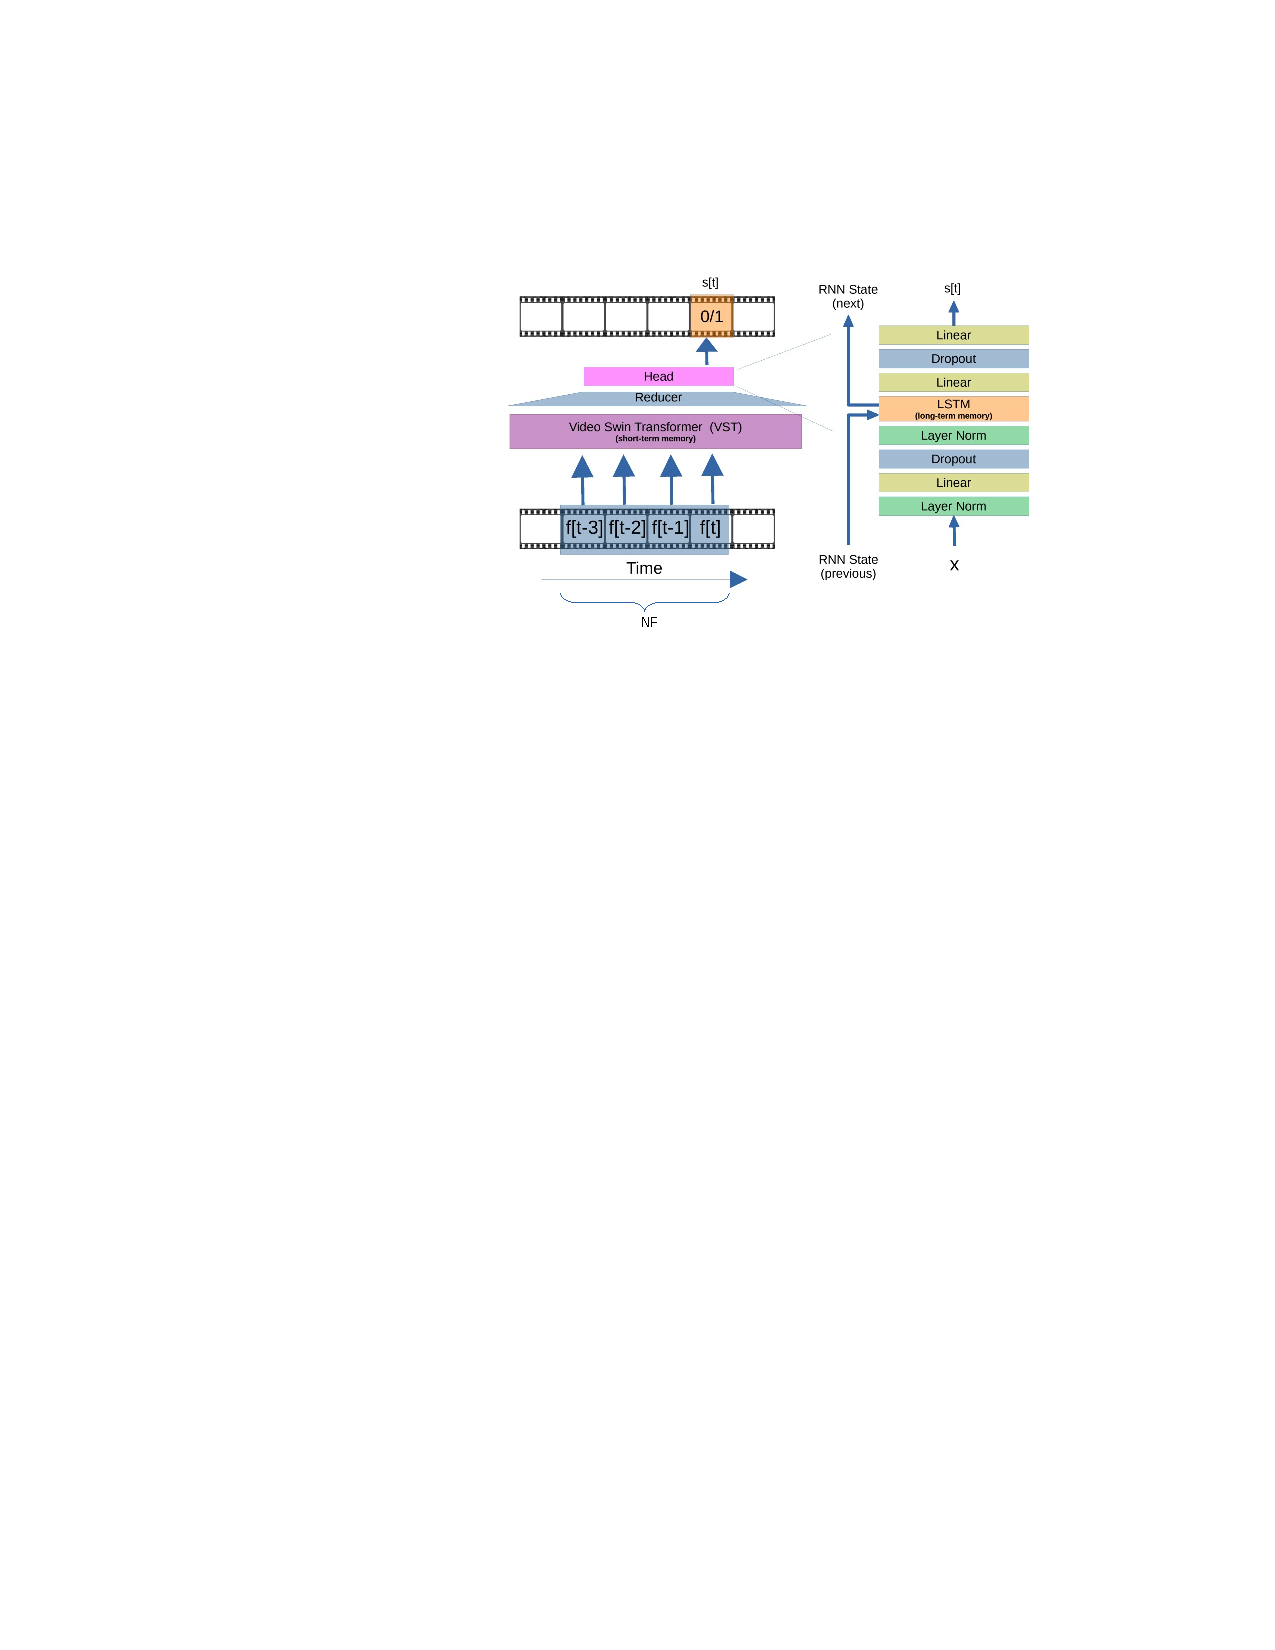
\includegraphics[trim=40 420 0 100, clip, width=1.\linewidth]{images/arch.pdf}
    %}
    % FIXME aggiungi link per immagine dei frame (copyriht)
    \caption{Video frame anomaly detection architecture.}
    \label{fig:arch}
\end{figure*}

In this section, the overall architecture shown in Figure \ref{fig:arch} will be exposed.
First, the Video Swin Trasformer \cite{liu_video_2022} model for the video action recognition task will be briefly described.
Then, the introduction of LSTM and the adaptation towards a real-time frame classification system will be described.
% TODO descrivere la nuova annotazione ??? Check motivazioni! :)

The Video Swin Transformer (VST) descends from Swin Transformer \cite{liu2021Swin}, which is a general-purpose image backbone with high performance on tasks that involve detection and localization.
The video extension takes in input a video with size $T \times H \times W \times 3$, where $T$, $H$ e $W$ correspond to number of frames, height and width, respectively.
The model split the video in non-overlapping 3D patches, partitioning the video in $\frac{T}{2} \times \frac{H}{4} \times \frac{W}{4}$ 3D tokens, projecting the features to an arbitrary dimension $C$.

Originally born to carry out the task of video action classification, it has been adapted to detect anomalies on single frame in a near-real time fashion, considering a temporal window of the latest three frames at time $t_{i-2}$, $t_{i-1}$ and $t_{i}$.
The output is computed in the following way:

\begin{equation}
\begin{split}
    r[t_{i}] &= Reducer(VST(f[t_{i-2}], f[t_{i-1}], f[t_{i}])) \\
    o[t_{i}] &= Cls(r[t_{i}], s[t_{i-1}])
\end{split}
\end{equation}

\noindent Where $f[t_{i-2}]$, $f[t_{i-1}]$ are the buffered past frames, $f[t_{i}]$ the current frame, $r[t_{i}]$ is the output of the reducer and $o[t_{i}]$ is the classification output of the frame at time $t_{i}$, $s[t_{i-1}]$ is the LSTM state.
The output of the $VST$ is collected and the number of channels is reduced by $Reducer$ (an Adaptive Average Pool 3D) and passed to the classifier $Cls$ composed by a three fully connected layers interspersed with a LSTM cell.
The LSTM cell was introduced to maintain a relationship between frames during training.
Past memory helps the classifier find connections to past frames out of reach of the transformer.

The final output $o[t_{i}]$ is the probability of the anomaly inside the last available frame $f[t_{i}]$.
This is trained with a weighted cross-entropy loss, giving more weight to the anomaly class, because it is spotted less frequently.

The final architecture and training modality are very simple and straightforward.
The use of the Transformer allows information to be extracted in a parallel and high-performance way with respect to an LSTM, on a limited number of frames which represents our short-term memory.
While, to keep information from the distant past as a long-term memory, we introduced an LSTM network interconnected to the classifier.
The choice of introduce it into the latent space of the classifier resulted in a limited additional computational cost.

% copyright image frame: <a href="https://www.freepik.com/free-vector/realistic-vector-icon-film-tape-strip-with-white-square-isolated-white-cinema-concept_31096470.htm#query=video%20frame&position=31&from_view=keyword">Image by user15245033</a> on Freepik